\documentclass{standalone}
\usepackage{tikz}
\usetikzlibrary{%                                                               
  shapes,arrows,positioning,decorations.markings,matrix,fit,tikzmark,           
  shapes.geometric,calc}
\tikzstyle{line} = [draw, -latex',line width=.7pt,fill=none]
\tikzstyle{dline} = [draw, latex'-latex',line width=.7pt,fill=none]
\definecolor{mBlue}{RGB}{4,110,152}
\definecolor{mGreen}{RGB}{115,180,85}
\definecolor{mYellow}{RGB}{230,195,35}
\definecolor{mOrange}{HTML}{EB811B}
\begin{document}
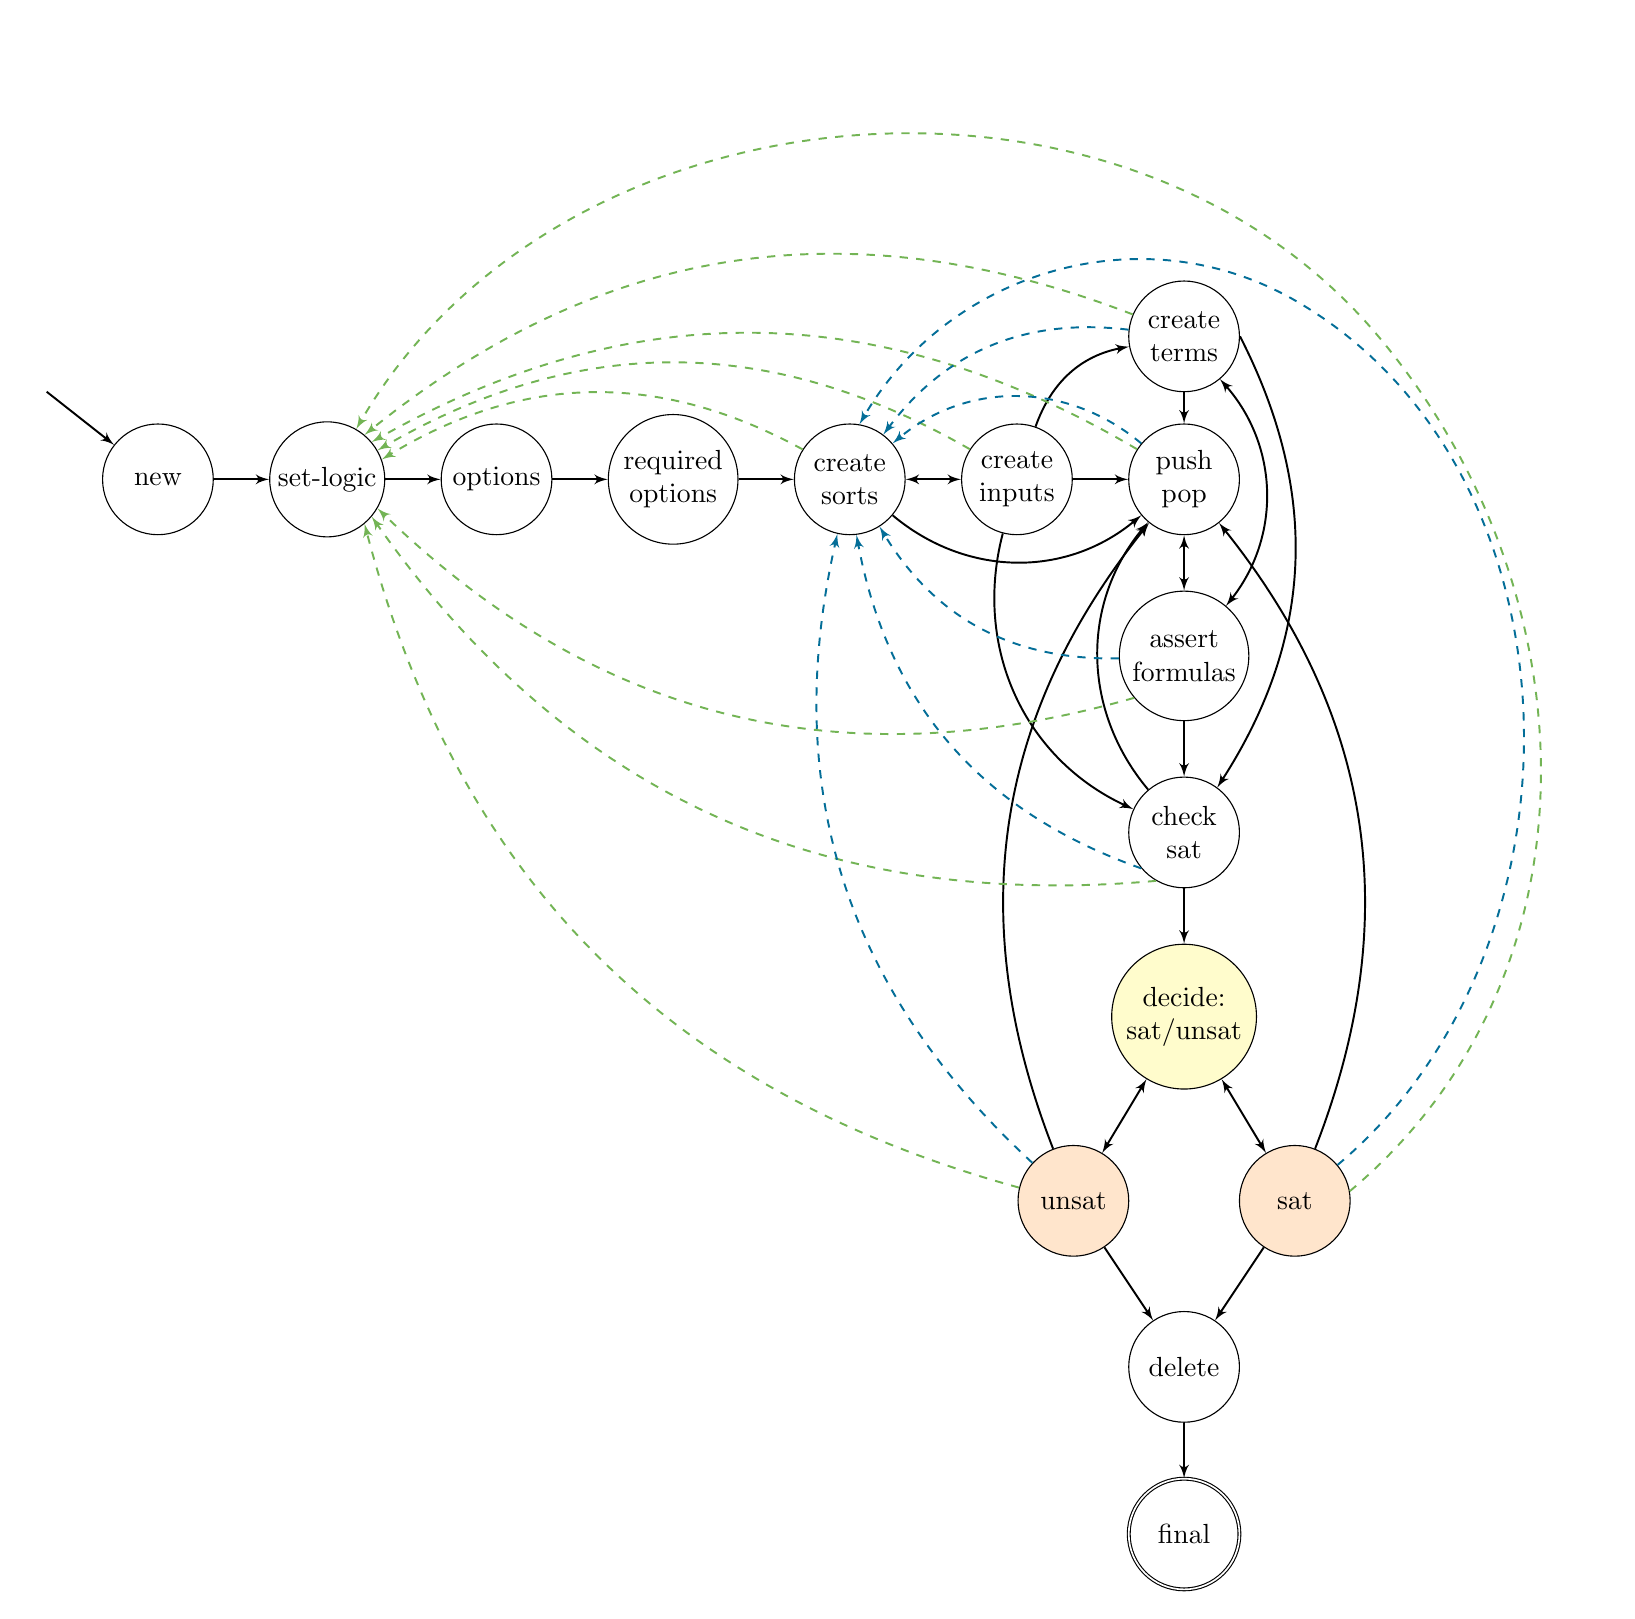
\begin{tikzpicture}[
    state/.style={
      draw,
      circle,
      minimum size=4.0em,
      fill=white,
      align=center,
      inner sep=2pt,
    },
    dstate/.style={
      draw,
      circle,
      minimum size=4.0em,
      fill=yellow!20,
      align=center,
      inner sep=2pt,
    },
    cstate/.style={
      draw,
      circle,
      minimum size=4.0em,
      fill=orange!20,
      align=center,
      inner sep=2pt,
    },
  ]

  \node[state] (new) {new};
  \node[left=2em of new, yshift=8ex] (start) {};
  \node[state,right=2em of new] (setlogic) {set-logic};
  \node[state,right=2em of setlogic] (opt) {options};
  \node[state,right=2em of opt] (optreq) {required\\options};
  \node[state,right=2em of optreq] (sorts) {create\\sorts};
  \node[state,right=2em of sorts] (inputs) {create\\inputs};
  \node[state,right=2em of inputs,yshift=12ex] (terms) {create\\terms};
  \node[state,right=2em of inputs] (pushpop) {push\\pop};
  \node[state,below=2em of pushpop] (assert) {assert\\formulas};
  \node[state,below=2em of assert] (checksat) {check\\sat};
  \node[dstate,below=2em of checksat] (dsat) {decide:\\sat/unsat};
  \node[cstate,below=2em of dsat,xshift=4em] (csat) {sat};
  \node[cstate,below=2em of dsat,xshift=-4em] (cunsat) {unsat};
  \node[state,below=8em of dsat] (delete) {delete};
  \node[state,below=2em of delete,double] (final) {final};

  \draw[line] (start) -- (new);
  \draw[line] (new) -- (setlogic);
  \draw[line] (setlogic) -- (opt);
  \draw[line] (opt) -- (optreq);
  \draw[line] (optreq) -- (sorts);
  \draw[dline] (sorts) -- (inputs);
  \path[draw,line] (sorts) to[bend right=40] (pushpop);

  %\draw[line] (inputs.200) -- (sorts.340);
  \path[draw,line] (inputs) to[bend left] (terms);
  \path[draw,line] (inputs) to[bend right=40] (checksat);
  \path[draw,line] (inputs) to (pushpop);

  %\path[draw,line] (terms) to[bend left=35] (assert);
  \path[draw,line] (terms.east) to[bend left] (checksat);
  \path[draw,line] (checksat) to[bend left=40] (pushpop);
  \draw[line] (terms) -- (pushpop);

  \path[draw,dline] (assert) to[bend right=40] (terms);
  \draw[line] (assert) -- (checksat);
  %\path[draw,line] (assert) to[bend left=40] (pushpop);

  \draw[line] (checksat) -- (dsat);
  \draw[dline] (dsat) -- (csat);
  \draw[dline] (dsat) -- (cunsat);

  \path[draw,line] (csat) to[bend right] (pushpop);
  %\path[draw,line] (csat) to[bend right] (checksat);
  \draw[line] (csat) -- (delete);

  \path[draw,line] (cunsat) to[bend left] (pushpop);
  %\path[draw,line] (cunsat) to[bend right] (checksat);
  \draw[line] (cunsat) -- (delete);

  \path[draw,dline] (pushpop) to (assert);

  \draw[line] (delete) -- (final);

  % reset
  \path[draw,line,mGreen,dashed] (sorts) to[bend right] (setlogic.20);
  \path[draw,line,mGreen,dashed] (inputs) to[bend right] (setlogic.30);
  \path[draw,line,mGreen,dashed] (pushpop) to[bend right] (setlogic.40);
  \path[draw,line,mGreen,dashed] (terms) to[bend right] (setlogic.50);
  \path[draw,line,mGreen,dashed] (csat.10)
     to[out=40,in=-50] ($(terms.east)+(5em,0ex)$)
     to[out=130,in=60] (setlogic.60);
  \path[draw,line,mGreen,dashed] (assert.220) to[bend left] (setlogic.330);
  \path[draw,line,mGreen,dashed] (checksat.240) to[bend left] (setlogic.320);
  \path[draw,line,mGreen,dashed] (cunsat) to[bend left] (setlogic.310);

  % reset assertions
  \path[draw,line,mBlue,dashed] (terms) to[bend right] (sorts);
  \path[draw,line,mBlue,dashed] (assert) to[bend left] (sorts);
  \path[draw,line,mBlue,dashed] (checksat.220) to[bend left] (sorts);
  \path[draw,line,mBlue,dashed] (cunsat) to[bend left] (sorts);
  \path[draw,line,mBlue,dashed] (csat.40)
     to[out=40,in=-30] ($(terms.east)+(2em,3ex)$) to[out=150,in=60] (sorts.80);

  \path[draw,line,mBlue,dashed] (pushpop) to[bend right=40] (sorts);

\end{tikzpicture}
\end{document}
